\section{Measurements of photon polarization in radiative decays}
\label{sec:photpol}
Radiative decays such as $\B^0_s \to \phi \gamma$ give access to information
about the photon polarization, and allow to test the presence of possible right-handed
couplings and set constraints on the Wilson coefficients $C_7$ and $C_7^{\prime}$ in EFT frameworks.
Previous measurements~\cite{} of photon polarization in radiative $B^0$ decays
have been compatible with SM predictions. 

LHCb is uniquely able to probe photon polarization in radiative $B^0_s$ decays,
which offer a complementary test of BSM physics. While a full analysis requires
tagging the production flavour of the $B^0_s$ meson, the large value of $\Delta\Gamma_s$
allows a measurement of the effective lifetime of $\B^0_s \to \phi \gamma$ to be
interpreted in terms of the $CP$-violating observable $A^\Delta$. LHCb
performs this measurement~\cite{} by normalizing the $\B^0_s \to \phi \gamma$ decay-time distribution
to that of $\B^0 \to K^{*0} \gamma$, cancelling most experimental biases on the decay-time.
The fitted mass and decay-time distributions are shown in Fig.~\ref{phigammamasstime}; LHCb finds
$A^\Delta = -0.98^{+0.46}_{-0.52}$, in $2\sigma$ agreement with the SM
prediction~\cite{} of $A^\Delta = 0.047 \pm 0.025 \pm 0.015$. The measurement is statistics
limited, and future tagged analyses will enable the (co)sinusoidal $CP$ observables to
be measured, allowing both the real and imaginary components of $C_7$ and $C_7^{\prime}$ to be constrained.

\begin{figure}
  \begin{center}
    \begin{tabular}{c c}
      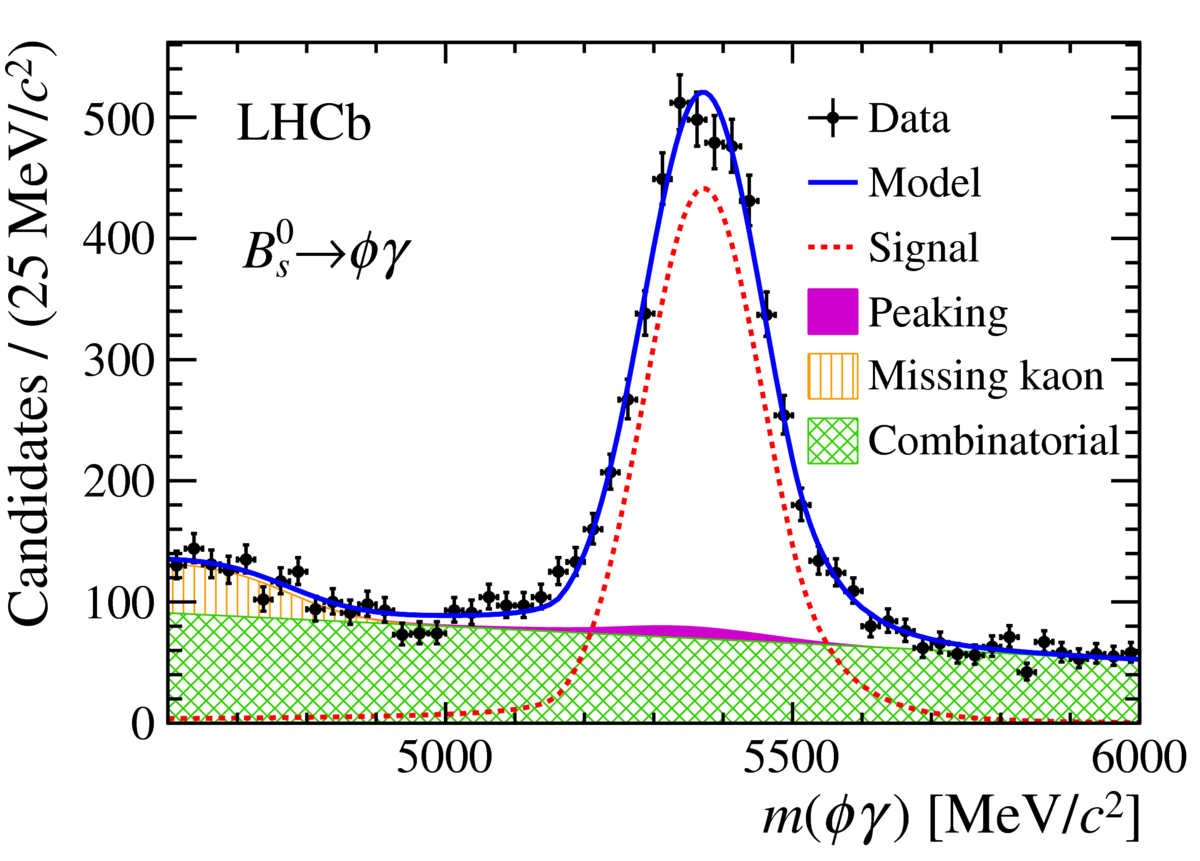
\includegraphics[height=5.5cm]{figs/phigammamass.png} &
      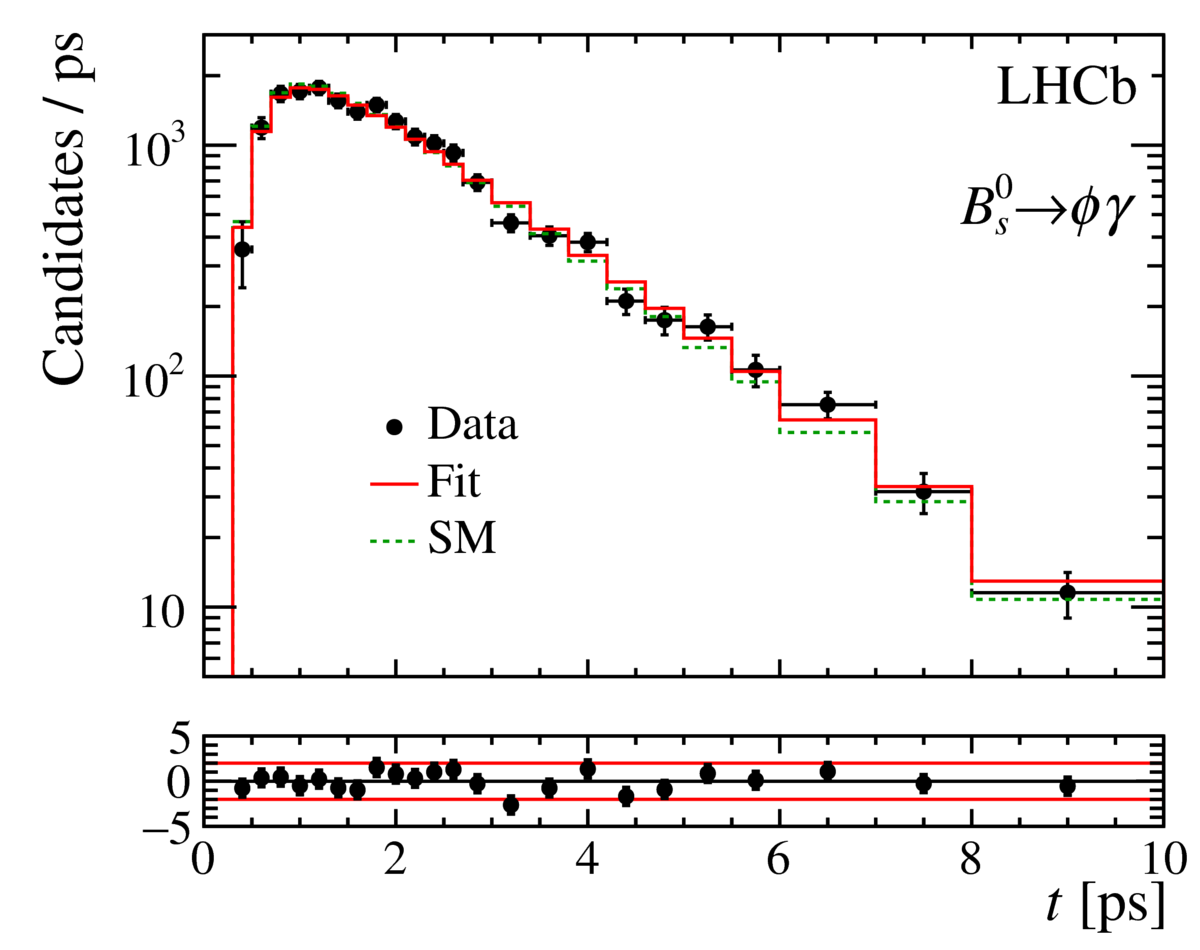
\includegraphics[height=5.5cm]{figs/phigammatime.png} 
    \end{tabular}
  \end{center}
  \vspace{-0.75cm}
  \caption{\label{phigammamasstime}Distributions of the fitted $\B^0_s \to \phi \gamma$ (left) invariant mass and (right) decay-time, reproduced from~\cite{}.}
\end{figure}
